\documentclass{article}
\usepackage{wrapfig}
\usepackage{graphicx}
\usepackage{textgreek}
\usepackage{amsmath}
\usepackage{caption}
\usepackage{geometry}
\usepackage{fancyhdr}
\usepackage{lastpage}
\geometry{
    a4paper,
    total={170mm,257mm},
    left=20mm,
    top=20mm,
}

\pagestyle{fancy}
\fancyhf{}
\fancyhead[RE,LO]{Name:}
\fancyfoot[RE,LO]{Gesamtpunktzahl: 14P}
\fancyfoot[LE,RO]{Seite \thepage/\pageref{LastPage}}

\graphicspath{ {./pictures/} }

\begin{document}

\part*{Aufgabe 2 - Spule mit Selbst- und Gegeninduktivität}

\begin{wrapfigure}{r}{0.3\textwidth}
\centering
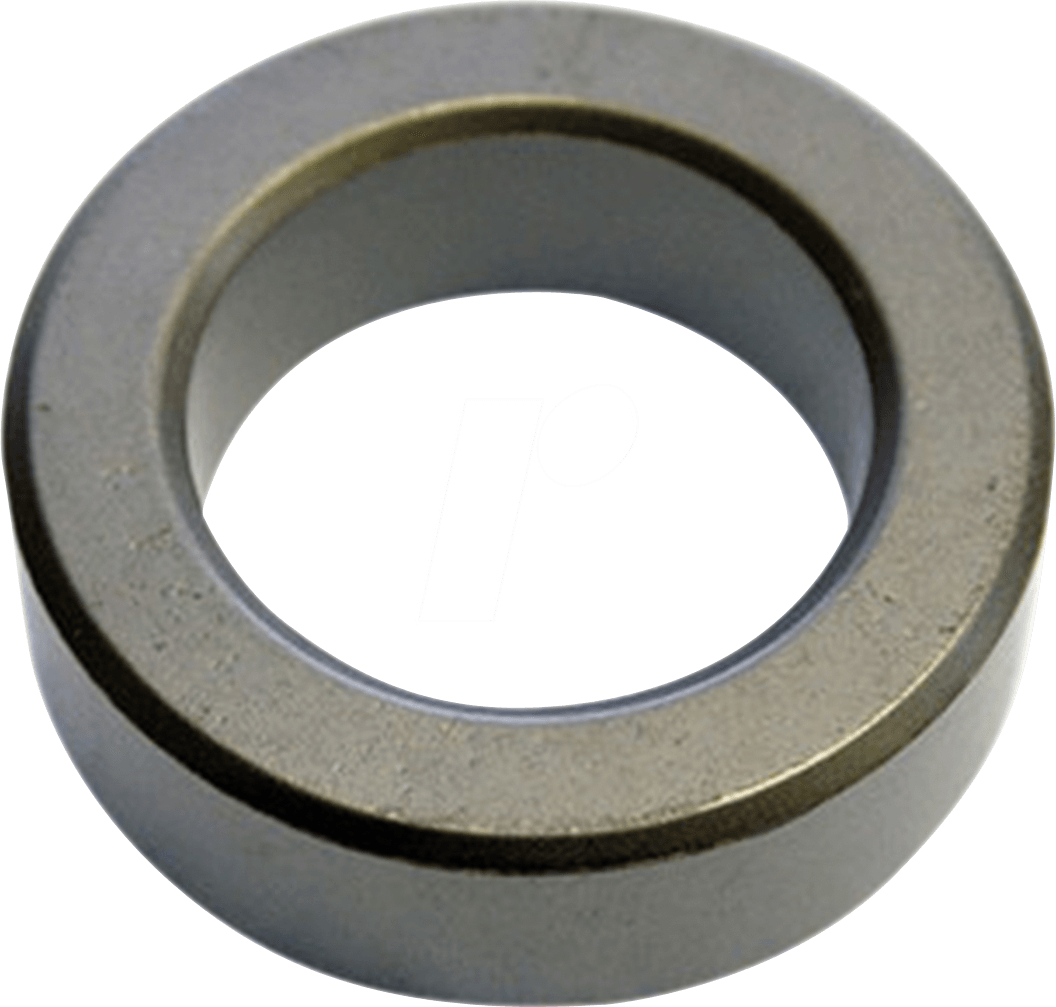
\includegraphics[width=.95\linewidth]{coil_core}
\caption*{Quelle: Reichelt}
\end{wrapfigure}
Ein Ring aus Ferrit (Annahme: $\mu_r = 2000$) mit kreisförmigem Querschnitt besitzt einen inneren Radius von $r_i = 10$mm und einen äußeren Radius von $r_a = 16$mm. Auf dem Ring sind zwei Wicklungen mit $N_1 = 150$ und $N_2 = 200$ Windungen mit gleichem Wicklungssinn angebracht.\\Gehen Sie von einem homogenen Feld im Inneren des Querschnitts aus. Streufelder sind zu vernachlässigen.\\
\subsection*{a) Berechnen Sie die Querschnittsfläche $A_q$ des Rings sowie die mittlere Feldlinienlänge $l$. (4P)}

\vspace{15mm}\vspace{15mm}
\subsection*{b) Wie groß ist der magnetische Widerstand $R_m$ der Anordnung? (2P)}

\vspace{15mm}
\subsection*{c) Wie groß sind die Induktivitäten $L_1$ und $L_2$ der Wicklungen? (3P)}

\vspace{15mm}\vspace{15mm}
\subsection*{d) Wie groß ist die Gegeninduktivität $M$? (5P)}

\vspace{15mm}


\end{document}
